\documentclass[conference]{IEEEtran}
\IEEEoverridecommandlockouts
% The preceding line is only needed to identify funding in the first footnote. If that is unneeded, please comment it out.
% \usepackage{cite}
% \bibliographystyle{IEEEtran}

\bibliographystyle{agsm} 
\usepackage{harvard}

\usepackage{amsmath,amssymb,amsfonts}
\usepackage{algorithmic}
\usepackage{graphicx}
\usepackage{textcomp}
\usepackage{xcolor}
\usepackage{float}

\usepackage{pifont} 
\usepackage{graphicx} % For \rotatebox
\usepackage{xcolor}
\usepackage{pifont}
\usepackage{booktabs}
\usepackage{amssymb} % for \checkmark
\usepackage{pifont}  % for \xmark
\usepackage{array}
\usepackage{multirow}

\usepackage{url}

\usepackage{dblfloatfix}  
\usepackage{multirow}

% Resolve figures from the comparison_output/figures directory and the paper root
% \graphicspath{{figures/}{./}}

% Define custom symbols
\newcommand{\cmark}{\textcolor{green!60!black}{\ding{51}}} % green tick
\newcommand{\xmark}{\textcolor{red}{\ding{55}}}            % red cross
\newcommand{\warn}{\textbf{--}} 



\def\BibTeX{{\rm B\kern-.05em{\sc i\kern-.025em b}\kern-.08em
    T\kern-.1667em\lower.7ex\hbox{E}\kern-.125emX}}
\begin{document}

\title{\textbf{PHLOP}: \textbf{P}hysics-Grounded \textbf{H}ierarchical \textbf{L}atent space for \textbf{O}bject
state and \textbf{P}resentation*\\
% {\footnotesize \textsuperscript{*}Note: Sub-titles are not captured in Xplore and
% should not be used}
% \thanks{Identify applicable funding agency here. If none, delete this.}
}

\author{\IEEEauthorblockN{1\textsuperscript{st} Mariia Zimokha}
\IEEEauthorblockA{\textit{School of Electronic Engineering and Computer Science} \\
\textit{Queen Mary University of London}\\
London, UK \\
0009-0004-2795-6739}
% \and
% \IEEEauthorblockN{2\textsuperscript{nd} Given Name Surname}
% \IEEEauthorblockA{\textit{dept. name of organization (of Aff.)} \\
% \textit{name of organization (of Aff.)}\\
% City, Country \\
% email address or ORCID}


}

\maketitle

\begin{abstract}
Understanding how objects move, interact, and respond to physical forces remains a key challenge in AI. Existing benchmarks such as CLEVRER, COMPHY, and Physion++ either rely on symbolic labels or lack interpretable grounding for physical dynamics. We introduce \textbf{PHLOP} (\textit{Physics-grounded Hierarchical Latent space for Object state and Presentation}), a diagnostic benchmark that bridges low-level physics and high-level reasoning. PHLOP uses MuJoCo simulations to procedurally generate diverse scenes with realistic object parameters (e.g., mass, friction, elasticity), and augments them with a hierarchical annotations defined by a formal taxonomy, covering different levels of abstraction of physical events (e.g., rolling, sliding, collision). Each video is annotated per-object, per-frame resolution. A question-generation module produces difficulty-graded queries spanning temporal, causal, and material reasoning over domain-generalization (out-of-distribution) splits. Experiments with open video-language models reveal substantial gaps in zero-shot physical understanding; parameter-efficient (LoRA) fine-tuning across difficulty curricula closes much of this gap, while textual physics hints help unevenly across models. PHLOP enables interpretable, reproducible, and fine-grained evaluation of physical reasoning and supports future research at the intersection of simulation and language.
\end{abstract}


\begin{IEEEkeywords}
simulation, physics engine, taxonomy, object properties, annotation, video question answering, visualization
\end{IEEEkeywords}



\section{Introduction}

\begin{table*}[!h]
\centering
\small
\setlength{\tabcolsep}{5pt}
\renewcommand{\arraystretch}{1.2}
\caption{
\textbf{Comprehensive Comparison of Physical Reasoning Benchmarks.}
PHLOP uniquely offers detailed Per-frame annotations defined by formal taxonomy, explicit friction and rotational dynamics modeling, and interpretable physical event detections. \textbf{Bold rows} highlight capabilities that are uniquely or fully supported by PHLOP. \cmark = fully supported, \warn = partially supported, \xmark = not supported.
}
\begin{tabular}{p{5.1cm}cccccccc}
\toprule
\textbf{Capability / Dataset} &
\textbf{PHLOP} &
\textbf{Physion++} &
\textbf{COMPHY} &
\textbf{CLEVRER} &
\textbf{ContPhy} &
\textbf{AGQA} &
\textbf{CATER} &
\textbf{PHYRE} \\
\midrule
\multicolumn{9}{l}{\textit{General Capabilities}} \\
Question Answering                   & \cmark & \cmark & \cmark & \cmark & \cmark & \cmark & \cmark & \xmark \\
Diagnostic Annotation                & \cmark & \warn  & \warn  & \warn  & \warn  & \xmark & \warn  & \warn \\
\textbf{Per-frame Annotations Defined by a Formal Taxonomy}   & \textbf{\cmark} & \xmark & \warn  & \xmark & \xmark & \xmark & \xmark & \xmark \\
Counterfactual Dynamics              & \cmark & \warn  & \warn  & \cmark & \warn  & \xmark & \xmark & \xmark \\
Explicit Physical Properties         & \cmark & \warn  & \warn  & \xmark & \warn  & \xmark & \xmark & \warn \\
Few-shot Material Reasoning          & \cmark & \warn  & \warn  & \xmark & \xmark & \xmark & \xmark & \xmark \\
\midrule
\multicolumn{9}{l}{\textit{Fine-Grained Physical Reasoning}} \\
Real-valued Properties (mass, friction, etc.) & \cmark & \warn & \warn & \xmark & \warn & \xmark & \xmark & \xmark \\
\textbf{Rotational Dynamics}         & \textbf{\cmark} & \xmark & \xmark & \xmark & \xmark & \xmark & \xmark & \xmark \\
\textbf{Friction-induced Events}     & \textbf{\cmark} & \xmark & \xmark & \xmark & \xmark & \xmark & \xmark & \xmark \\
\textbf{Elastic vs. Inelastic Collision} & \textbf{\cmark} & \warn  & \warn  & \xmark & \xmark & \xmark & \xmark & \xmark \\
\textbf{Moving Event Onset Detection}  & \textbf{\cmark} & \xmark & \xmark & \xmark & \xmark & \xmark & \xmark & \xmark \\
\textbf{Distribution-based Material Sampling} & \textbf{\cmark} & \warn  & \warn  & \xmark & \xmark & \xmark & \xmark & \xmark \\
\bottomrule
\end{tabular}
\label{tab:phlop_full_comparison}
\end{table*}


Physical reasoning, which involves understanding and predicting how objects interact, move, and respond to forces, is fundamental to both human cognition and machine intelligence \cite{yi2020clevrer,tung2023physion++,battaglia2013simulation,piloto2022intuitive}. From an early age, humans intuitively grasp complex physical interactions \cite{piloto2022intuitive,battaglia2013simulation}. For instance, when watching a ball bounce off the floor, people naturally expect it to slow down or bounce back depending on its elasticity, even without explicit calculations \cite{battaglia2013simulation,piloto2022intuitive}. 
Despite rapid advances in deep learning, AI models continue to struggle with structured and interpretable physical reasoning \cite{tung2023physion++,battaglia2013simulation,piloto2022intuitive,melnik2023benchmarks,physicsrw2024}.
Bridging this gap is crucial for applications in robotics, computer vision, and AI, where models must interpret dynamic scenes and make physically plausible predictions \cite{yi2020clevrer,tung2023physion++,battaglia2013simulation}. 



% Existing benchmarks such as CLEVRER~\cite{yi2020clevrer}, COMPHY~\cite{chen2022comphy}, and Physion++~\cite{tung2023physion++} have advanced model evaluation significantly, but remain limited in their interpretability and semantic grounding.


Existing benchmarks, such as CLEVRER \cite{yi2020clevrer}, COMPHY \cite{chen2022comphy}, and Physion++ \cite{tung2023physion++}, have significantly advanced our ability to evaluate models on tasks of physical reasoning; however, each comes with its limitations. 
CLEVRER relies on symbolic labels for events (e.g., ``collision'') that lack explicit physical grounding, making it challenging to analyze fine-grained dynamics \cite{yi2020clevrer}. COMPHY enhances interpretability through compositional physical concepts while simplifying physics by excluding rotational dynamics and approximating friction modeling \cite{chen2022comphy}. Physion++ integrates a wide range of physical properties and scene diversity, yet it lacks per-frame annotations and event-level semantic labeling, limiting interpretability for temporal and causal analysis \cite{tung2023physion++}.

% However, they face limitations in either relying on abstract symbolic events (e.g., high-level labels like "collision" without underlying physical parameters) or focusing on raw dynamics (e.g., trajectories, forces), which lack semantic grounding, making it challenging to align model predictions with human-understandable concepts \cite{tung2023physion++,piloto2022intuitive,melnik2023benchmarks}. 

% Recent work in this area highlights this disconnect, which prevents models from inferring mechanical properties (e.g., friction, elasticity) in human-interpretable terms \cite{tung2023physion++,physicsrw2024}. 
Recent work highlights this disconnect, as models struggle to infer latent physical properties from purely visual cues \cite{hofherr2023neural} 
% \cite{ physicsinverse2024, physicsguided2023}
, or match human-level physical reasoning \cite{benchmarkingInfant2024}.
For instance, while a physics engine may simulate a bouncing ball using precise coefficients, humans describe the same event in qualitative terms: ``the ball bounces high because it is very elastic'' \cite{battaglia2013simulation,piloto2022intuitive}.


To address these limitations, we introduce \textbf{PHLOP} (Physics-Grounded Hierarchical Latent space for Object state and Presentation), a novel benchmark and data set developed from the ground up. PHLOP unifies detailed physical simulation with structured semantic annotations to support hierarchical reasoning over dynamic physical events. Our key contributions include:
\begin{itemize}

\item \textbf{Physics-grounded Dataset}: PHLOP is a novel benchmark that provides per-object, per-frame data generated from rigid-body simulations. It includes rich physical attributes (e.g., mass, velocity, friction, elasticity) and frame-aligned annotations of physical events grounded in continuous dynamics.

\item \textbf{Hierarchical physical taxonomy}: We design a structured taxonomy that captures multiple levels of abstraction, from low-level motion and contact dynamics to high-level events, enabling interpretability and flexible supervision.


\item \textbf{Semantic-Physical Alignment}:
PHLOP maps numerical physical behaviors to interpretable labels, bridging the gap between low-level physics and high-level reasoning tasks.

\item \textbf{Domain-generalization splits}: PHLOP is partitioned into \textsc{train}/\textsc{val}/\textsc{test} sets whose generative factors (shapes, materials and their physical sub-components, object counts, collision modes, floor textures, and camera profiles) are deliberately disjoint, so evaluation measures out-of-distribution generalization rather than memorization.

\item \textbf{Difficulty-graded questions}: Each generated question is annotated with a difficulty label (\textit{easy}/\textit{medium}/\textit{hard}/\textit{very\_hard}) reflecting the depth of reasoning required, enabling curriculum-based analysis.


\item \textbf{Model evaluation and learning analysis}: We evaluate open video-language models both zero-shot and under LoRA fine-tuning, with and without textual physics hints, characterizing how curriculum composition and non-visual cues shape physical reasoning.

\item \textbf{Reproducible Simulation Framework}: The project includes a GitHub repository that enables the generation of new scenes with controllable physics. PHLOP provides a reproducible method for creating and recreating specific scenes with various object properties and conditions.

\end{itemize}

% This paper introduces the PHLOP dataset, describing its structure, taxonomy, simulation platform, and evaluation tools. Our goal is to provide a benchmark that not only supports learning physical dynamics but also connects these dynamics to interpretable, language-grounded reasoning. PHLOP fills a critical gap in the landscape of physical reasoning benchmarks by aligning with both the numerical fidelity of physics engines and the semantic richness needed for human-like understanding.

\section{Related Work}


Recent years have seen significant progress in developing datasets that support the study and evaluation of machine understanding of object dynamics, causal structure, and intuitive physics in videos \cite{yi2020clevrer,tung2023physion++}. These benchmarks can be categorized as (i) symbolic diagnostic benchmarks, (ii) physics-grounded simulations, and (iii) video-based reasoning task. We briefly review each and position PHLOP within this landscape.

\subsection{Symbolic Diagnostic Benchmarks}

The early dataset, such as CLEVR \cite{johnson2017clevr} and CLEVRER~\cite{yi2020clevrer}, primarily focused on symbolic or template-based reasoning.
CLEVR \cite{johnson2017clevr} established a structured visual question-answering (VQA) system involving object attributes (e.g., ``Is there a red cube to the left of the blue sphere?'') using photos of synthetic scenes, but due to its nature, it lacked temporal or physical dynamics.
CLEVRER \cite{yi2020clevrer} was built on this idea and pioneered video-based causal and counterfactual question answering, around object collisions and motion on the surface. For instance, ``What caused the red ball to stop?'' or ``What would happen if the green object were removed?''. However, physical interactions are abstracted into high-level symbolic labels (e.g., ``collide'') without grounding in continuous physical parameters , limiting their utility for fine-grained physical analysis \cite{yi2020clevrer}. 
Answers to diagnostic questions remain symbolic, lacking annotations that are defined by a formal taxonomy and cover different levels of abstraction, or explicit physical properties to explain causality.
IntPhys \cite{riochet2018intphys} introduced violations of intuitive physics, and CRAFT \cite{wu2020craft} incorporated causal reasoning with forces, but both rely on categorical abstractions rather than physically grounded measures.

\subsection{Physics-Grounded Simulations}

To move beyond symbolic abstraction, recent benchmarks have incorporated physics engines to generate realistic dynamics. PHYRE \cite{bakhtin2019phyre} provides a library of 2D physical puzzle scenes governed by gravity, where tasks involve predicting outcomes under known initial conditions. However, PHYRE does not expose object-level physical parameters such as friction or mass.

 
ComPhy \cite{chen2022comphy} expands the scope to more complex 3D multi-object dynamics, supporting compositional physical reasoning (e.g., removing an object and re-simulating). However, it has limited material diversity, representing materials with categorical labels, and simplifies physics by assuming uniform friction and omitting rotational dynamics and distribution-based sampling of physical parameters.

Physion++ \cite{tung2023physion++} further extends these approaches, introducing complex interactions and scene diversity by varying object properties (e.g., size, shape, density) and simulation types (rigid, fluid, deformable). It focuses on high-level prediction tasks (e.g., ``Will the object fall off the table?'') rather than detailed physical analysis, and lacks structured semantic grounding of events or per-frame physical state labels \cite{tung2023physion++}. 

Recent approaches like SuperCLEVR~\cite{superclevr2024} and PhysGen~\cite{physgen2024} explore procedural video generation and physics-based prediction, but do not provide per-frame, object-level semantic labels as PHLOP does. InfLevel~\cite{piloto2022infant} measures model surprise under physically implausible conditions (e.g., gravity violation), offering developmental psychology-inspired diagnostics but not per-object tracking.


ContPhy \cite{zhang2024contphy} proposes attribute-based scene analysis (e.g., object softness or size) in physically consistent environments. While this supports high-level reasoning, it does not offer per-frame semantic annotations. Hofherr et al.~\cite{hofherr2023neural} explore real-valued parameter estimation using neural implicit functions, and Liu et al.~\cite{physicsinverse2024} frame physical parameter estimation as an inverse-graphics problem. Both works highlight the need for interpretable, structured metadata like that in PHLOP.

\subsection{Video Reasoning Datasets}
Some datasets approach physical reasoning as part of general video understanding. CATER \cite{girdhar2019cater} focuses on object permanence and spatial tracking under occlusion, but uses simple 3D object shuffles without realistic physics. AGQA \cite{grunde2021agqa} scales video QA to real-world scenes, asking about action sequences and object interactions, but relies on high-level semantic cues rather than low-level physical simulation. While these datasets advance multi-modal understanding, they are not designed to explore questions requiring physical causality, material properties, or dynamical system behavior.


% Some datasets approach physical reasoning as part of general video understanding. 
% CATER \cite{girdhar2019cater} focuses on object permanence and spatial tracking under occlusion, but uses simple 3D object shuffles without realistic physics. 
% AGQA \cite{grunde2021agqa} scales video QA to real-world scenes, asking about action sequences and object interactions, but relies on high-level semantic cues rather than low-level physical simulation. 
% Both datasets target spatio-temporal reasoning but lack physical fidelity. 


More recent efforts such as Helping Hands \cite{helpinghands2023}, Learning Object States \cite{learningObjectStates2023}, and disentangled SDE dynamics \cite{disentangleSDE2023} contribute to object-centric video reasoning, highlighting temporal dependencies and state changes in visual data. 
While these datasets advance multimodal understanding, they are not designed to explore questions requiring physical causality, material properties, or dynamical system behavior—domains where PHLOP aims to bridge the gap.


\subsection{PHLOP in Context}


Recent work leverages procedural priors for scene generation and video prediction~\cite{takenaka2023procedural}, suggesting that control over simulation parameters can guide model learning. 
The design of PHLOP is also inspired by theoretical foundations: simulation-based cognition \cite{battaglia2013simulation}, intuitive physics learning \cite{piloto2022intuitive}, and physics-guided machine learning \cite{physicsguided2023}. Reference material properties are grounded in established engineering and physics resources \cite{ashby2018engineering,callister2020materials,halliday2013physics}, ensuring physical realism in the dataset.  
PHLOP builds on these advances while addressing critical limitations in existing physical reasoning datasets. Table~\ref{tab:phlop_full_comparison} outlines how the dataset uniquely bridges low-level dynamics and high-level semantics.

% t uniquely bridges low-level dynamics and high-level semantics, as systematically outlined in Table~\ref{tab:phlop_full_comparison}.


% Unlike CLEVRER’s symbolic abstraction, PHLOP provides continuous-valued physical parameters (e.g., mass, friction) that ground reasoning in measurable reality. COMPHY improves interpretability via compositional scenes but lacks friction modeling, rotational motion, and real-valued physical attributes—all of which are explicitly modeled in PHLOP. Physion++ introduces physical diversity, but lacks per-frame semantic labels, frictional reasoning, and interaction-level taxonomy.

% Unlike \textbf{CLEVRER}’s\cite{yi2020clevrer} symbolic approach, PHLOP provides continuous physical parameters  (e.g., mass, friction). \textbf{COMPHY}\cite{chen2022comphy} improves interpretability via compositional scenes but lacks friction modeling, rotational motion, and real-valued physical attributes—all of which are explicitly modeled in PHLOP. \textbf{Physion++}\cite{tung2023physion++} introduces physical diversity, but lacks per-frame semantic labels, frictional reasoning, and interaction-level classification.

% In contrast to \textbf{AGQA}\cite{grunde2021agqa} and \textbf{CATER}\cite{girdhar2019cater}, which focus on high-level scene understanding or action tracking, PHLOP emphasizes physical causality and low-level interaction analysis. While \textbf{PHYRE}\cite{bakhtin2019phyre} offers interactive prediction tasks, it does not support per-frame annotation  organized by a formal taxonomy, or material property inference.


PHLOP uniquely enables:

\begin{itemize}
    \item \textbf{Per-frame semantic labeling} of object states and transitions—absent in all prior benchmarks.
    \item \textbf{Rotational and frictional event detection}, such as rolling, slipping, or friction-induced halts.
    \item \textbf{Elastic vs. inelastic collision analysis} using velocity changes and energy loss metrics.
    \item \textbf{Few-shot material reasoning} via continuous distribution-based sampling across density, elasticity, and friction.
    \item \textbf{Moving event onset detection}, allowing frame-accurate identification of motion transitions.
\end{itemize}



These capabilities enable novel types of questions such as: 
\begin{itemize}
    \item ``Which object experienced the greatest kinetic energy loss?''
    \item ``When did the red ball stop rolling?''
\end{itemize}


Such queries require the unified physical and semantic grounding that prior datasets lack. By combining continuous dynamics with interpretable labels, PHLOP offers a scalable, diagnostic benchmark for evaluating grounded physical reasoning in vision-language models.


\section{Methodology}
 In this section, we describe the creation of PHLOP, which involves two core components: (1) the dataset creation process for generating physics-accurate videos with ground truth annotations, and (2) the benchmark evaluation framework for assessing video-language models on physical reasoning tasks.


% \vspace{-1.9em} 

\subsection{Dataset Creation}

  
\subsubsection{Video Generation Process}
\begin{figure*}[h]
\centering
\begin{tabular}{ccc}
\includegraphics[width=0.3\linewidth]{images/col -sliding-rolling/1.png} &
\includegraphics[width=0.3\linewidth]{images/col -sliding-rolling/2.png} &
\includegraphics[width=0.3\linewidth]{images/col -sliding-rolling/3.png} \\
\includegraphics[width=0.3\linewidth]{images/col -sliding-rolling/4.png} &
\includegraphics[width=0.3\linewidth]{images/col -sliding-rolling/5.png} &
\includegraphics[width=0.3\linewidth]{images/col -sliding-rolling/6.png} \\
\end{tabular}
\caption{Sequence of 6 frames showing dynamic object interactions and taxonomy-based annotations in the PHLOP simulation. Each frame captures per-object motion, material properties, and physical events.}
\label{fig:phlop_frames}
\end{figure*}


PHLOP contains roughly 20{,}000 generated videos - partitioned into 16{,}000 \textsc{train}, 2{,}000 \textsc{val}, and 2{,}000 \textsc{test} scenes (Section~\ref{sec:splits})- each depicting a simulated physical scene involving multiple rigid objects with varying properties and interactions.

Scenes are created using the MuJoCo physics engine~\cite{todorov2012mujoco}. Each scene involves one or more physical events such as collisions, sliding, rolling, or frictional deceleration. The simulation captures these interactions at a high resolution of $1024 \times 768$ pixels at 25 FPS, capturing dense temporal sequences of interactions. This object-centric logging bridges physical reasoning and visual understanding by aligning data with physical ground truth.

The dataset is generated using a controlled randomization method over object attributes (shape, size, color), physical properties (e.g., friction and restitution), and initial conditions (e.g., velocity vectors, spatial configurations). 

\subsubsection{Semantic Annotation and Taxonomy}

Physical events within each video are annotated automatically at the frame and object level using PHLOP’s hierarchical taxonomy. This taxonomy categorizes interactions across several abstraction levels:
\begin{itemize}
    \item \textbf{Level 1:} Broad physical category (e.g., Kinematic Events)
    \item \textbf{Level 2:} Event type (e.g., Rotational Motion)
    \item \textbf{Level 3:} Fine-grained label (e.g., Rolling with Slipping)
\end{itemize}


Table~\ref{tab:phlop_taxonomy_clean} defines this taxonomy. It allows PHLOP to support taxonomy-based prompting and structured question generation.


% Annotations are derived from simulation logs using rules over motion thresholds, velocity changes, and force-based triggers. For example, an object labeled as ``Friction Stop'' must meet criteria for velocity approaching zero under non-collisional deceleration.
Annotations are derived from simulation logs using rules over motion thresholds, velocity changes, and force-based triggers. For example, an object labeled as ``Friction Stop'' must meet criteria for velocity approaching zero under non-collisional deceleration. Collisions are further graded by the fraction of kinetic energy retained, yielding \textit{Elastic}, \textit{Partially Inelastic}, and \textit{Highly Inelastic} labels rather than a single binary category.




\noindent\textbf{Shape-aware detection.}
Event detection is conditioned on object geometry, since the same kinematic signature implies different physical events for different shapes. Spheres are eligible for rotational labels (rolling, slipping) but are excluded from sliding-friction detection, whereas cubes and blocks are treated as sliding contacts. Cylinders are handled according to their instantaneous orientation: an \emph{upright} cylinder (resting on a flat end) is evaluated for sliding-friction events, while a cylinder lying on its side is evaluated for rotational motion (rolling and rolling-with-slipping).


\begin{table*}[!t]
\centering
\renewcommand{\arraystretch}{1.3}
\setlength{\tabcolsep}{6pt}
\caption{
Hierarchical taxonomy of physical events in PHLOP. Events are organized into general categories (Level 1), subcategory types (Level 2), and specific event labels (Level 3). Collisions are graded into three energy-based classes; rotational and friction events are detected with shape- and orientation-aware rules.}
\label{tab:phlop_taxonomy_clean}
\begin{tabular}{|>{\raggedright\arraybackslash}m{4.2cm}|>{\raggedright\arraybackslash}m{4.2cm}|>{\raggedright\arraybackslash}m{6.8cm}|}
\hline
\textbf{Level 1 (General Category)} & \textbf{Level 2 (Event Type)} & \textbf{Level 3 (Specific Event Labels)} \\
\hline
\multirow{7}{*}{\textbf{Kinematic Events}} 
 & Linear Motion          & Constant Velocity \\
 &                        & Decelerating \\
 &                        & Accelerating \\
 &                        & Stationary \\
 & Rotational Motion      & Pure Rotation \\
 &                        & Rolling Motion \\
 &                        & Rolling Motion with Slipping \\
\hline
\multirow{3}{*}{\textbf{Interaction Events}} 
 & Collisions             & Elastic Collision \\
 &                        & Partially Inelastic Collision \\
 &                        & Highly Inelastic Collision \\
\hline
\multirow{2}{*}{\textbf{State Transitions}} 
 & Motion Change          & Moving to Stopping \\
 &                        & Stationary to Moving \\
\hline
\multirow{2}{*}{\textbf{Environmental Interactions}} 
 & Friction-Induced Events & Friction Stop (Stopped Due to Friction) \\
 &                         & Sliding with Friction \\
\hline
\end{tabular}
\end{table*}



% \subsubsection{Parameter Sampling}
% To ensure both visual and physical diversity, PHLOP samples a range of object-level and global scene parameters. Tables~\ref{tab:material_physical} and~\ref{tab:scene_params} summarize the full range of material and scene properties used.


% \begin{table}[H]
% \centering
% \renewcommand{\arraystretch}{1.6}
% \setlength{\tabcolsep}{2pt}
% \caption{Material physical properties with real-world reference values~\cite{ashby2018engineering,callister2020materials}.}
% \label{tab:material_physical}
% \begin{tabular}{|l|c|c|c|p{2.2cm}|}
% \hline
% \textbf{Material} & \textbf{Elasticity} (–) & \textbf{Density} (kg/m$^3$) & \textbf{Friction} (–) & \textbf{Examples} \\
% \hline
% Metal   & 0.85–0.92 & 2700–19320 & 0.28–0.32 & Steel, Aluminum, Copper \\
% Wood    & 0.35–0.45 & 500–700    & 0.45–0.55 & Softwood, Hardwood \\
% Rubber  & 0.90–0.98 & 900–1200   & 0.90–1.10 & Natural, Synthetic \\
% Glass   & 0.55–0.65 & 2400–2600  & 0.18–0.22 & Soda-lime, Borosilicate \\
% Plastic & 0.65–0.75 & 1000–1800  & 0.35–0.45 & LDPE, PP, PC \\
% \hline
% \end{tabular}
% \end{table}


\subsubsection{Parameter Sampling}

To ensure both visual and physical diversity, PHLOP samples a range of object-level and global scene parameters. Tables~\ref{tab:material_physical} and~\ref{tab:scene_params} summarize the full range of material and scene properties used.


\begin{table}[H]
\centering
\renewcommand{\arraystretch}{1.6}
\setlength{\tabcolsep}{2pt}
\caption{Material physical properties with real-world reference values~\protect\cite{ashby2018engineering,callister2020materials}.}
\label{tab:material_physical}
\begin{tabular}{|l|c|c|c|p{2.2cm}|}
\hline
\textbf{Material} & \textbf{Elasticity} (–) & \textbf{Density} (kg/m$^3$) & \textbf{Friction} (–) & \textbf{Examples} \\
\hline
Metal   & 0.85–0.92 & 2700–19320 & 0.28–0.32 & Steel, Aluminum, Copper \\
Wood    & 0.35–0.45 & 500–700    & 0.45–0.55 & Softwood, Hardwood \\
Rubber  & 0.90–0.98 & 900–1200   & 0.90–1.10 & Natural, Synthetic \\
Glass   & 0.55–0.65 & 2400–2600  & 0.18–0.22 & Soda-lime, Borosilicate \\
Plastic & 0.65–0.75 & 1000–1800  & 0.35–0.45 & LDPE, PP, PC \\
\hline
\end{tabular}
\end{table}



% \vspace{-.5em}  



% \begin{table}[H]
% \centering
% \renewcommand{\arraystretch}{1.5} % Increase row height
% \setlength{\tabcolsep}{5.5pt}       % Adjust horizontal cell padding (default is 6pt)

% \footnotesize 
% \caption{Material physical properties with representative density values}
% \label{tab:material_physical}
% \begin{tabular}{|l|c|c|c|p{1.5cm}|}
% \hline
% \textbf{Material} & \textbf{Elasticity (unitless)} & \textbf{Density (kg/m$^3$)} & \textbf{Friction (unitless)} & \textbf{Primary Density Types} \\
% \hline
% Metal   & 0.85--0.92 & 2700--19320 & 0.28--0.32 & Steel, Aluminum, Copper \\
% Wood    & 0.35--0.45 & 500--700    & 0.45--0.55 & Softwood, Hardwood \\
% Rubber  & 0.90--0.98 & 900--1200   & 0.90--1.10 & Natural, Synthetic \\
% Glass   & 0.55--0.65 & 2400--2600  & 0.18--0.22 & Soda-lime, Borosilicate \\
% Plastic & 0.65--0.75 & 1000--1800  & 0.35--0.45 & LDPE, PP, PC \\
% \hline
% \end{tabular}
% \end{table}

% \begin{table}[h]
% \centering
% \caption{Material visual properties}
% \begin{tabular}{|l|c|c|c|l|}
% \hline
% \textbf{Material} & \textbf{Alpha} & \textbf{Specular} & \textbf{Shininess} & \textbf{Visual Characteristics} \\
% \hline
% Glass   & 0.5 & 0.6 & 50  & Semi-transparent with reflections \\
% Metal   & 1.0 & 1.0 & 100 & Opaque with high reflectivity \\
% Wood    & 1.0 & 0.2 & 10  & Opaque with low reflectivity \\
% Rubber  & 1.0 & 0.0 & 0   & Opaque with no reflectivity \\
% Plastic & 1.0 & 0.3 & 5   & Opaque with moderate reflectivity \\
% \hline
% \end{tabular}
% \end{table}


% \begin{table}[H]
% \centering
% \renewcommand{\arraystretch}{1.5} % Increase row height
% \setlength{\tabcolsep}{4pt} 

% \caption{Global scene parameter specifications}
% \label{tab:scene_params}
% \begin{tabular}{|l|p{3.5cm}|p{3.0cm}|}
% \hline
% \textbf{Component} & \textbf{Parameter Range} & \textbf{Description} \\
% \hline
% Camera & \textbf{Lookat}: $[-0.5,0.5] \times [-0.5,0.5] \times [-0.5,0.5] $, \textbf{Distance}: 1.5--3.5\,m & Camera position in 3D space \\
%        & \textbf{Azimuth}: $[-90^\circ, -30^\circ]$, \textbf{Elevation}: $[-30^\circ, 0^\circ]$ & Viewing angle constraints \\
% Lighting & \textbf{Position}: $[-1,1] \times [-1,1] \times [0.1,0.7]$ & Lighting position in 3D space \\
%          & \textbf{Diffuse}: 0.7--1.0, \textbf{Specular}: 0.5--1.0 & Light intensities \\
%          & \textbf{Cutoff}: $50^\circ$--$180^\circ$ & Angular spread \\
% Floor & \textbf{Friction}: Static [0.0,1.0], Dynamic $\leq$ Static & Three-component friction \\
%       & \textbf{Specular}: 0.2--0.8, \textbf{Shininess}: 0.2--0.8 & Visual settings \\
%       & \textbf{RGBA}: brightness  & Color mapping \\
% \hline
% \end{tabular}
% \end{table}
% \vspace{-.5em}  

% \noindent\textbf{Material Physical Properties:}
% Table~\ref{tab:material_physical} presents material-specific property ranges with representative real-world context.
% Each object in the simulation is assigned properties that determine its physical behavior and visual appearance. Sampling was performed from the material-specific distributions that can be found in  Table~\ref{tab:material_physical}.  Each object is assigned:


\noindent\textbf{Material Physical Properties:}
Table~\ref{tab:material_physical} presents material-specific property ranges with representative real-world context.
Each object in the simulation is assigned properties that determine its physical behavior and visual appearance. Sampling was performed from the material-specific distributions that can be found in  Table~\ref{tab:material_physical}.  Each object is assigned:
\begin{itemize}
    \item \textbf{Shape}: Chosen randomly from \texttt{sphere}, \texttt{cube}, \texttt{cylinder}, or \texttt{block}, each with different moments of inertia and contact surfaces.
    \item \textbf{Material Type}: Samples randomly from a discrete set (e.g., \texttt{wood}, \texttt{metal}, \texttt{rubber}, \texttt{glass}, \texttt{plastic}), each associated with different parameter distributions.
    \item \textbf{Physical Properties:} Material-dependent distributions for density, elasticity, and friction (Table~\ref{tab:material_physical}).
    \item \textbf{Visual Properties:} Material-specific transparency, specularity, shininess, and random color.
    \item \textbf{Dimensions:} Ball/cylinder radius 0.05--0.1m, cube side 0.05--0.1m, block 0.01--0.1m $\times$ 0.05--0.1m $\times$ 0.05--0.1m.
    \item \textbf{Initial Position \& Orientation}: Randomized in 3D space to create spatial variability across simulations.
    \item \textbf{Mass:} Calculated from volume and sampled density, minimum 1e-6 kg.
    \item \textbf{Initial Velocities:} Linear velocities are sampled in meters per second (m/s) and angular velocities in radians per second (rad/s). They uniformly sampled in 3D space $[-1,1] \times [-1,1] \times [-1,1], (x,y,z)$.
\end{itemize}

% \begin{itemize}
%     \item \textbf{Shape}: Chosen randomly from \texttt{sphere}, \texttt{cube}, \texttt{cylinder}, or \texttt{block}, each with different moments of inertia and contact surfaces.
%     \item \textbf{Material Type}: Samples randomly from a discrete set (e.g., \texttt{wood}, \texttt{metal}, \texttt{rubber}, \texttt{glass}, \texttt{plastic}), each associated with different parameter distributions.
%     \item \textbf{Physical Properties:} Material-dependent distributions for density, elasticity, and friction (Table~\ref{tab:material_physical}).
%     \item \textbf{Visual Properties:} Material-specific transparency, specularity, shininess, and random color.
%     \item \textbf{Dimensions:} Ball/cylinder radius 0.05--0.1m, cube side 0.05--0.1m, block 0.01--0.1m $\times$ 0.05--0.1m $\times$ 0.05--0.1m.
    
%     \item \textbf{Initial Position \& Orientation}: Randomized in 3D space to create spatial variability across simulations.
%     \item \textbf{Mass:} Calculated from volume and sampled density, minimum 1e-6 kg.
    
%     % \item \textbf{Initial Velocities:} Linear and angular velocities uniformly sampled in 3D space $[-1,1] \times [-1,1] \times [-1,1], (x,y,z)$.

%     \item \textbf{Initial Velocities:} Linear velocities are sampled in meters per second (m/s) and angular velocities in radians per second (rad/s). They uniformly sampled in 3D space $[-1,1] \times [-1,1] \times [-1,1], (x,y,z)$.

% \end{itemize}

% \begin{table}[t]
% \centering
% \renewcommand{\arraystretch}{1.5} % Increase row height
% \setlength{\tabcolsep}{4pt} 

% \caption{Global scene parameter specifications}
% \label{tab:scene_params}
% \begin{tabular}{|l|p{3.5cm}|p{3.0cm}|}
% \hline
% \textbf{Component} & \textbf{Parameter Range} & \textbf{Description} \\
% \hline
% Camera & \textbf{Lookat}: $[-0.5,0.5] \times [-0.5,0.5] \times [-0.5,0.5] $, \textbf{Distance}: 1.5--3.5\,m & Camera position in 3D space \\
%        & \textbf{Azimuth}: $[-90^\circ, -30^\circ]$, \textbf{Elevation}: $[-30^\circ, 0^\circ]$ & Viewing angle constraints \\
% Lighting & \textbf{Position}: $[-1,1] \times [-1,1] \times [0.1,0.7]$ & Lighting position in 3D space \\
%          & \textbf{Diffuse}: 0.7--1.0, \textbf{Specular}: 0.5--1.0 & Light intensities \\
%          & \textbf{Cutoff}: $50^\circ$--$180^\circ$ & Angular spread \\
% Floor & \textbf{Friction}: Static [0.0,1.0], Dynamic $\leq$ Static & Three-component friction \\
%       & \textbf{Specular}: 0.2--0.8, \textbf{Shininess}: 0.2--0.8 & Visual settings \\
%       & \textbf{RGBA}: brightness  & Color mapping \\
% \hline
% \end{tabular}
% \end{table}
\begin{table}[t]
\centering
\renewcommand{\arraystretch}{1.5}
\setlength{\tabcolsep}{4pt} 
\caption{Global scene parameter specifications}
\label{tab:scene_params}
\begin{tabular}{|l|p{3.5cm}|p{3.0cm}|}
\hline
\textbf{Component} & \textbf{Parameter Range} & \textbf{Description} \\
\hline
Camera & \textbf{Lookat}: $[-0.5,0.5] \times [-0.5,0.5] \times [-0.5,0.5] $, \textbf{Distance}: 1.5--3.5\,m & Camera position in 3D space \\
       & \textbf{Azimuth}: $[-90^\circ, -30^\circ]$, \textbf{Elevation}: $[-30^\circ, 0^\circ]$ & Viewing angle constraints \\
Lighting & \textbf{Position}: $[-1,1] \times [-1,1] \times [0.1,0.7]$ & Lighting position in 3D space \\
         & \textbf{Diffuse}: 0.7--1.0, \textbf{Specular}: 0.5--1.0 & Light intensities \\
         & \textbf{Cutoff}: $50^\circ$--$180^\circ$ & Angular spread \\
Floor & \textbf{Friction}: Static [0.0,1.0], Dynamic $\leq$ Static & Three-component friction \\
      & \textbf{Specular}: 0.2--0.8, \textbf{Shininess}: 0.2--0.8 & Visual settings \\
      & \textbf{RGBA}: brightness  & Color mapping \\
\hline
\end{tabular}
\end{table}
% \end{table}

% \vspace{-.5em} 

\noindent\textbf{Global Scene Parameters:}
Table~\ref{tab:scene_params} provides comprehensive specifications for environmental factors:
\begin{itemize}
    \item \textbf{Lighting:} 
    \textit{Position}, \textit{color}, \textit{reflectivity}, and \textit{angular spread} control the directionality and softness of shadows and highlights.
    \item \textbf{Camera:} 
    \textit{Azimuth} and \textit{elevation} define the viewing angle; \textit{distance} and \textit{look-at point} control framing and focus.
    \item \textbf{Floor Plane:} 
    \textit{Friction coefficient}, \textit{color} (based on friction), \textit{shininess}, and \textit{specular reflectance} are sampled to vary how objects interact with surfaces visually and physically.
\end{itemize}



\begin{figure*}[h]
\centering
\begin{tabular}{cc}
\includegraphics[width=0.48\linewidth]{images/sliding/1.png} &
\includegraphics[width=0.48\linewidth]{images/sliding/2.png} \\
\includegraphics[width=0.48\linewidth]{images/sliding/3.png} &
\includegraphics[width=0.48\linewidth]{images/sliding/4.png} \\
\end{tabular}
\caption{Sequence of 4 frames showing dynamic object interactions and taxonomy-based annotations in the PHLOP simulation.}
\label{fig:phlop_4frames}
\end{figure*}
All parameters—both global and per-object—are stored alongside the simulation for full reproducibility and analysis. These attributes drive the emergence of behaviors such as gliding, bouncing, tumbling, and frictional halts, allowing PHLOP to capture a comprehensive range of Newtonian phenomena.


\subsubsection{Dataset Splits for Domain Generalization}
\label{sec:splits}
To evaluate \emph{generalization} rather than memorization, PHLOP is partitioned into \textsc{train}, \textsc{val}, and \textsc{test} splits whose generative factors are deliberately \emph{disjoint}. Rather than randomly partitioning a single pool of scenes - which would let a model exploit shared textures, materials, or viewpoints - each split draws from a different region of the scene parameter space: distinct object shapes, materials, per-material physical sub-components (e.g.\ different metal alloys), object-count ranges, collision modes, floor textures, and camera profiles. Consequently, a model is tested on material--shape--viewpoint combinations it never saw during training (e.g.\ \texttt{rubber} and \texttt{block} objects under an ``extreme'' camera profile appear \emph{only} in the test split). Table~\ref{tab:splits} summarizes the configuration. Because the sub-components are also disjoint, even shared material categories (e.g.\ \texttt{glass}) use different physical-parameter regions across splits.
\begin{table}[t]
\centering
\caption{Disjoint generative factors per split, enforcing out-of-distribution evaluation. Material sub-components (e.g.\ metal alloys) are also disjoint across splits, so even shared material categories use different physical-parameter regions.}
\label{tab:splits}
\small
\begin{tabular}{llll}
\toprule
Factor & Train & Val & Test \\
\midrule
Shapes        & ball, cube, cyl.     & ball, cube         & block, cyl., cube \\
Materials     & metal, wood, plastic & metal, wood, glass & glass, rubber \\
\#Objects     & 2--6                 & 2--5               & 3--7 \\
Camera        & broad                & narrow             & extreme \\
Collisions    & coll./slide/stat.    & coll./slide        & coll./offset/slide \\
Floor         & checker/flat         & flat/gradient      & checker/gradient \\
\bottomrule
\end{tabular}
\end{table}
Every scene is additionally rendered under two \textbf{camera modes}---a \texttt{static} fixed-viewpoint render and a \texttt{moving} (orbiting) render---allowing the same physical event to be probed under different visual coverage. All experiments reported here use the \texttt{static} mode for a controlled, single-viewpoint comparison; one trade-off of this fixed viewpoint is that some events can fall outside the frame or behind an occluder, rendering a fraction of questions unanswerable from the static view (quantified and handled in Section~\ref{sec:finetune-results}).

The figures~\ref{fig:phlop_frames} and~\ref{fig:phlop_4frames} illustrate different scenes from the dataset, where the number of objects and environmental conditions vary. Notably, the camera position and lighting conditions differ between the two scenes. The taxonomy annotations also reflect different physical interactions. Figure~\ref{fig:phlop_frames} shows a more complex scenario involving an inelastic collision, where a moving object interacts with a stationary one, causing it to move. In contrast, Figure~\ref{fig:phlop_4frames} presents a simpler case, where two objects slide and eventually stop due to friction.


%     \item \textbf{Mass and Density}: Sampled per material type using realistic statistical priors. For instance, metal objects have higher density and mass variance than rubber.
%     \item \textbf{Elasticity (Restitution)}: Real-valued coefficients (typically 0.1–0.9) control how much kinetic energy is retained during collisions.
%     \item \textbf{Friction Coefficient}: Sampled from material-dependent ranges (e.g., high for rubber, low for metal), affecting sliding, rolling, and stopping behavior.
%     \item \textbf{Initial Position \& Orientation}: Randomized in 3D space to create spatial variability across simulations.
%     \item \textbf{Initial Velocity \& Angular Velocity}: Objects may start at rest or with translational/rotational motion, sampled from controlled distributions to elicit rich dynamical outcomes.
% \end{itemize}

% All parameters—both global and per-object—are stored alongside the simulation for full reproducibility and analysis. These attributes drive the emergence of behaviors such as gliding, bouncing, tumbling, and frictional halts, allowing PHLOP to capture a comprehensive range of Newtonian phenomena.



% These attributes are encoded and stored per instance to ensure reproducibility and enable fine-grained comparative evaluation.


\subsubsection{Verification and Quality Assurance}
To ensure visual-semantic alignment and correctness of the annotations, each simulation produces three video modalities: RGB video, segmentation video (with object-specific masks), and annotated video (with bounding boxes, physical attributes, and semantic event labels). These were used to manually verify that physical events, object identities, and interaction dynamics were captured correctly across time.
While most annotations are generated algorithmically from simulation logs using rule-based logic, a sampled subset of the generated dataset was manually reviewed to validate consistency. For example, rolling events were cross-checked against angular and linear velocity curves, or stationary objects were checked whether linear velocity is approximately zero within a threshold. Future work may explore using learned classifiers to automate this verification at scale.


% \subsubsection{Verification and Quality Assurance}
% To ensure visual-semantic alignment and correctness of the annotations, each simulation produces three video modalities: RGB video, segmentation video (with object-specific masks), and annotated video (with bounding boxes, physical attributes, and semantic event labels). These were used to manually verify that physical events, object identities, and interaction dynamics were captured correctly across time.

% While most annotations are generated algorithmically from simulation logs using rule-based logic, approximately 5\% of the generated dataset (\textasciitilde 200 videos) was manually reviewed to validate consistency. For example, rolling events were cross-checked against angular and linear velocity curves, or stationary objects were checked whether linear velocity is approximately zero within a threshold. Future work may explore using learned classifiers to automate this verification at scale.

% While most annotations are generated algorithmically from simulation logs using rule-based logic, a portion of the dataset was manually reviewed to validate consistency. For example, rolling events were cross-checked against angular and linear velocity curves, or stationary objects were checked whether linear velocity is approximately zero within a threshold. Future work may explore using learned classifiers to automate this verification at scale.


\subsection{Benchmark Methodology}


\subsubsection{Automatic Question Generation}
PHLOP includes a built-in module for automatic question generation based on the annotated physical interactions and object properties.  This module leverages simulation logs (mass, velocity, position, etc.) and per-frame taxonomy labels to create grounded question-answer pairs. Questions are designed to test a spectrum of reasoning skills, including:
\begin{itemize}
    \item \textbf{Temporal Reasoning}: e.g., ``At what time does the red ball become stationary?''
    \item \textbf{Material Property Inference}: e.g., ``Which object had the highest friction coefficient?''
    \item \textbf{Interaction and Outcome}:
          e.g., ``Which object was involved in the most collisions?''
    \item \textbf{Aggregate Events}: e.g., ``How many objects rolled during the video?''
    \item \textbf{Energy \& Loss}: e.g., ``What percentage of system kinetic energy was lost in a collision?''
\end{itemize}

Unlike symbolic QA in CLEVRER~\cite{yi2020clevrer}, PHLOP's questions are grounded in both semantic labels and physical data. This allows richer evaluation of model understanding across symbolic, causal, and physical domains. The questions and the respective correct answers are unambiguous because of their grounding in the simulation data, enabling evaluation of both the language and the compositional physical understanding.


\subsubsection{Question Difficulty Annotation}
\label{sec:difficulty}
Each automatically generated question is tagged with a \textbf{difficulty} label---\textit{easy}, \textit{medium}, \textit{hard}, or \textit{very\_hard}---reflecting the depth of reasoning required rather than surface form. The label is assigned by the question generator from the underlying reasoning type:
\begin{itemize}
  \item \textbf{Easy}: single-step perception and counting (object count, rolling detection, stopped-object count, collision presence).
  \item \textbf{Medium}: property comparison and attribute inference (e.g.\ highest-friction object, velocity/friction scaling).
  \item \textbf{Hard} / \textbf{very\_hard}: multi-step physical reasoning over continuous dynamics (momentum/energy conservation, multi-hop causation, temporal-event ordering).
\end{itemize}
These labels are the basis of the fine-tuning curriculum in Section~\ref{sec:finetune}.


\subsubsection{Prompt Construction and Types}
\label{sec:prompt-types}

Across both zero-shot and fine-tuning evaluation, each model receives 32 uniformly sampled frames, an instruction on how to answer, and a question with multiple-choice options, under one of two prompting settings:
\begin{enumerate}
    \item \textbf{No physics hint}: video and question only; no metadata is included.
    \item \textbf{With physics hint}: object-specific physical parameters are appended to the prompt, such as:
    \begin{quote}
      \textbf{\textit{``1. darkcyan sphere: mass = 0.8, friction = 0.92''}}
    \end{quote}
\end{enumerate}
Critically, the physics hint provides contextual cues but not the correct answer; it lists parameters for \emph{all} objects--including those irrelevant to the current question---introducing distractors so that the model must focus on the relevant information and reason compositionally rather than retrieve a fact. Comparing the two settings isolates how much each model relies on textual physical cues versus grounded visual dynamics, in the spirit of the structured-context analyses of Physion++~\cite{tung2023physion++} and ContPhy~\cite{zhang2024contphy}.



\subsubsection{Fine-tuning Protocol and Difficulty Ablation}
\label{sec:finetune}
We  \textbf{LoRA-fine-tune} three open vision--language models---\textbf{SmolVLM}, \textbf{Qwen2-VL}, and \textbf{InternVL3} - on PHLOP, to see how the mix of question difficulties used for training affects physical reasoning. We train four versions of each model that differ only in which difficulties they are trained on (Table~\ref{tab:ftconfig}): \textit{easy}, \textit{easy+medium}, \textit{hard}, or \textit{full} (all difficulties). While a model is training, we track its accuracy on the difficulties it was \emph{not} trained on and use that to decide when to stop. We then test every model- and the original zero-shot model -on the test set, and this test set includes questions of \emph{all} difficulties. In other words, the curriculum name only says what a model was \emph{trained} on; all models are \emph{tested} on the same complete test set (Section~\ref{sec:finetune-results}). This lets us measure two kinds of generalization: to new scenes (new materials, shapes, and camera views; Table~\ref{tab:splits}) and to question difficulties the model never saw in training (Table~\ref{tab:ftconfig}).

\begin{table}[t]
\centering
\caption{The four fine-tuning setups. Each one trains on a different set of question difficulties. The ``Validation difficulties'' (the ones left out of training) are used only to decide when to stop training. Every setup is then tested on the same test set, which includes all difficulties.}

\label{tab:ftconfig}
\small
\begin{tabular}{lll}
\toprule
Curriculum & Train difficulties & Validation difficulties \\
\midrule
\textit{easy}         & easy         & medium, hard, very\_hard \\
\textit{easy\_medium} & easy, medium & hard, very\_hard \\
\textit{hard}         & hard         & easy, medium, very\_hard \\
\textit{full}         & all          & --- (no holdout) \\
\bottomrule
\end{tabular}
\end{table}
Each curriculum is run under the two prompting settings of Section~\ref{sec:prompt-types} (no physics hint / with physics hint). Together with the non-fine-tuned \emph{zero-shot} baseline, this yields five conditions per model and prompting setting, all evaluated on the same held-out \textsc{test} split of $25{,}436$ questions (a fraction of which are unanswerable from the static viewpoint; Section~\ref{sec:finetune-results}). Results are reported in Section~\ref{sec:finetune-results}.


\section{Results}
\label{sec:finetune-results}

We report accuracy exactly as produced by the official PHLOP evaluator on the held-out \textsc{test} split. For every model we compare five conditions---the non-fine-tuned \emph{zero-shot} baseline plus the four LoRA curricula of Table~\ref{tab:ftconfig} (\textit{easy}, \textit{easy+medium}, \textit{hard}, and \textit{full}/all-tasks)---each under the two prompting settings of Section~\ref{sec:prompt-types} (no physics hint / physics-augmented). Beyond a single overall score, the evaluator also reports accuracy separately for each \emph{test-question difficulty} (Easy, Medium, Hard, Very hard), which lets us see not only \emph{how much} fine-tuning helps but \emph{where} it helps.

\paragraph{Static-camera caveat.}
All experiments use the \texttt{static} (fixed-viewpoint) render, so the difficulty ablation is a like-for-like comparison under one camera. A side effect is that a small fraction of questions ($\approx 11\%$) refer to an object or event that the fixed viewpoint does not capture---it happens off-screen or behind an occluder---making them effectively unanswerable from the static view; this is a matter of camera coverage, not reasoning. Rendering the same scenes with the \texttt{moving} (orbiting) camera would recover many of these cases and is left to future work.

\subsection{Overall Model Performance}

Table~\ref{tab:finetune-ablation} reports overall accuracy for all three models across the five conditions and both prompting settings, and Figure~\ref{fig:overall-heatmap} shows the complete picture broken down by test-question difficulty. Three findings stand out. First, \textbf{zero-shot physical reasoning is weak}: without fine-tuning, the models score between $17.8\%$ and $32.9\%$ overall---at or near chance for the multiple-choice format---confirming that off-the-shelf VLMs do not solve PHLOP. Second, \textbf{LoRA fine-tuning closes most of this gap}: the best configuration reaches $91.2\%$ for InternVL3, $88.3\%$ for SmolVLM, and $64.0\%$ for the more brittle Qwen2-VL. Third, the \textbf{best curriculum is model-dependent}: SmolVLM peaks under the all-tasks (\textit{full}) curriculum, whereas InternVL3 and Qwen2-VL peak marginally under \textit{easy+medium} ($92.0\%$ and $68.2\%$ with hints), with \textit{full} a close second. The difficulty breakdown in Figure~\ref{fig:overall-heatmap} also reveals a counter-intuitive pattern: after fine-tuning, the \emph{Hard} and \emph{Very hard} tiers are often answered at near-ceiling accuracy (InternVL3 exceeds $99\%$ on \emph{Hard} and reaches $100\%$ on \emph{Very hard}), while the \emph{Easy} tier lags (e.g.\ $71.7\%$ for InternVL3 without hints). The human-oriented \emph{difficulty} labels (reasoning depth) therefore do not track empirical model difficulty: the hardest-labelled tiers are dominated by templates the models learn to answer reliably, whereas some ``easy'' perception and counting questions remain visually challenging.

\begin{table*}[t]
\centering
\caption{\textbf{Overall accuracy (\%) on the held-out test set}, as reported by the official PHLOP evaluator, for the zero-shot baseline and the four LoRA curricula, with and without physics hints. Column names denote the difficulties each model was \emph{trained} on; every model is \emph{tested} on the same full test set (all difficulties). A per-difficulty breakdown is given in Figure~\ref{fig:overall-heatmap}. \textbf{Bold} marks the best condition per row.}
\label{tab:finetune-ablation}
\small
\begin{tabular}{llrrrrr}
\toprule
Model & Physics hint & Baseline & Easy & Easy+Med & Hard & Full \\
\midrule
\multirow{2}{*}{SmolVLM}   & No  & 32.89 & 65.68 & 72.72 & 60.50 & \textbf{84.36} \\
                           & Yes & 32.93 & 70.36 & 79.99 & 59.08 & \textbf{88.33} \\
\midrule
\multirow{2}{*}{Qwen2-VL}  & No  & 22.64 & 19.99 & 46.01 & 37.30 & \textbf{51.64} \\
                           & Yes & 17.79 & 44.83 & \textbf{68.17} & 50.66 & 64.04 \\
\midrule
\multirow{2}{*}{InternVL3} & No  & 24.00 & 65.56 & \textbf{86.00} & 84.38 & 84.23 \\
                           & Yes & 22.68 & 68.29 & \textbf{92.03} & 88.48 & 91.16 \\
\bottomrule
\end{tabular}
\end{table*}



\begin{figure*}[t]
    \centering
    
\includegraphics[width=0.95\textwidth]{heatmap_absolute_accuracy.pdf}
    \caption{\textbf{Fine-tuning accuracy across task difficulty} (official evaluator, \% correct; higher is better). Rows are curricula (baseline plus the four training sets); columns are the overall score and the four test-question difficulty tiers; the left block is physics-augmented, the right block no-physics. Fine-tuning on all tasks gives consistently high accuracy across tiers, and the hardest tiers are answered at near-ceiling once fine-tuned.}
    \label{fig:overall-heatmap}
\end{figure*}


\subsection{Curriculum Dependence}

Since every model is tested on the same test set and the curricula differ only in their \emph{training} difficulties, Figures~\ref{fig:radar-permodel} and~\ref{fig:radar-macro} show how the choice of training difficulties reshapes accuracy across the difficulty tiers. Training on \emph{all} tasks (\textit{full}) gives the broadest coverage: its polygon is outermost or tied on nearly every axis for every model, and it dominates especially on the \emph{Hard} and \emph{Very hard} tiers. Narrow curricula transfer unevenly. A model trained only on \textit{hard} questions becomes excellent on the \emph{Hard} tier (e.g.\ SmolVLM $97.8\%$, Qwen2-VL $98.0\%$) but collapses on \emph{Medium} and \emph{Very hard}, so its overall score is mediocre. Conversely, \textit{easy+medium} is a strong all-rounder---for InternVL3 and Qwen2-VL it slightly edges \textit{full} overall---because the bulk of the test set falls in the easier tiers. The models also differ in robustness. InternVL3 generalizes well even from a narrow slice (trained only on \textit{hard}, it still reaches $84.4\%$ overall without hints). Qwen2-VL is the most fragile: trained on \textit{easy} only without hints it scores just $20.0\%$ overall---below its own $22.6\%$ baseline---so a too-narrow curriculum can actively hurt a weak backbone. Averaged over the three models (Figure~\ref{fig:radar-macro}), the ordering is clear and consistent: \textit{full} $\gtrsim$ \textit{easy+medium} $>$ \textit{hard} $>$ \textit{easy} $\gg$ baseline.



\begin{figure*}[t]
    \centering
    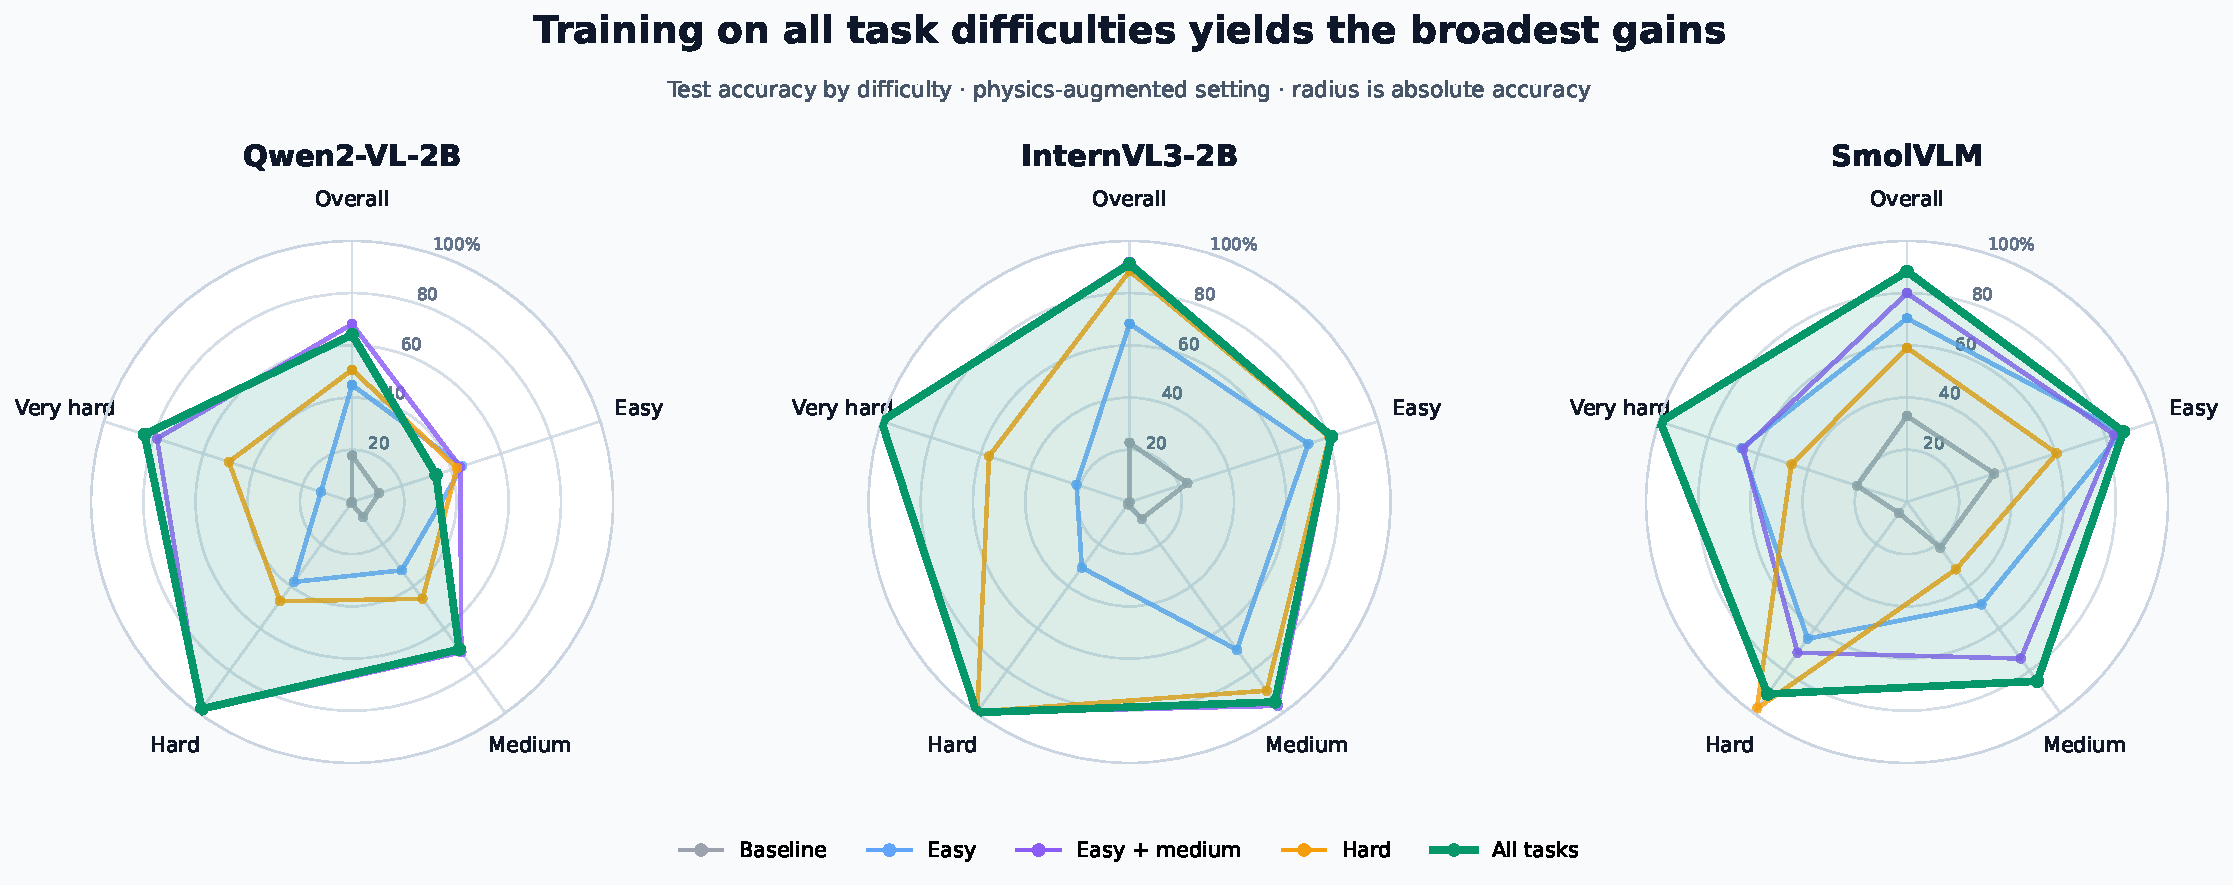
\includegraphics[width=0.98\textwidth]{radar_finetuning_comparison_with_physics.pdf}
    \caption{\textbf{Per-model accuracy by difficulty (physics-augmented).} Each panel is one model; the axes are the overall score and the four difficulty tiers; each polygon is a training curriculum. Training on all tasks (green) gives the broadest coverage. The no-physics version is in Figure~\ref{fig:radar-permodel-nophys}.}
    \label{fig:radar-permodel}
\end{figure*}

\begin{figure}[t]
    \centering
    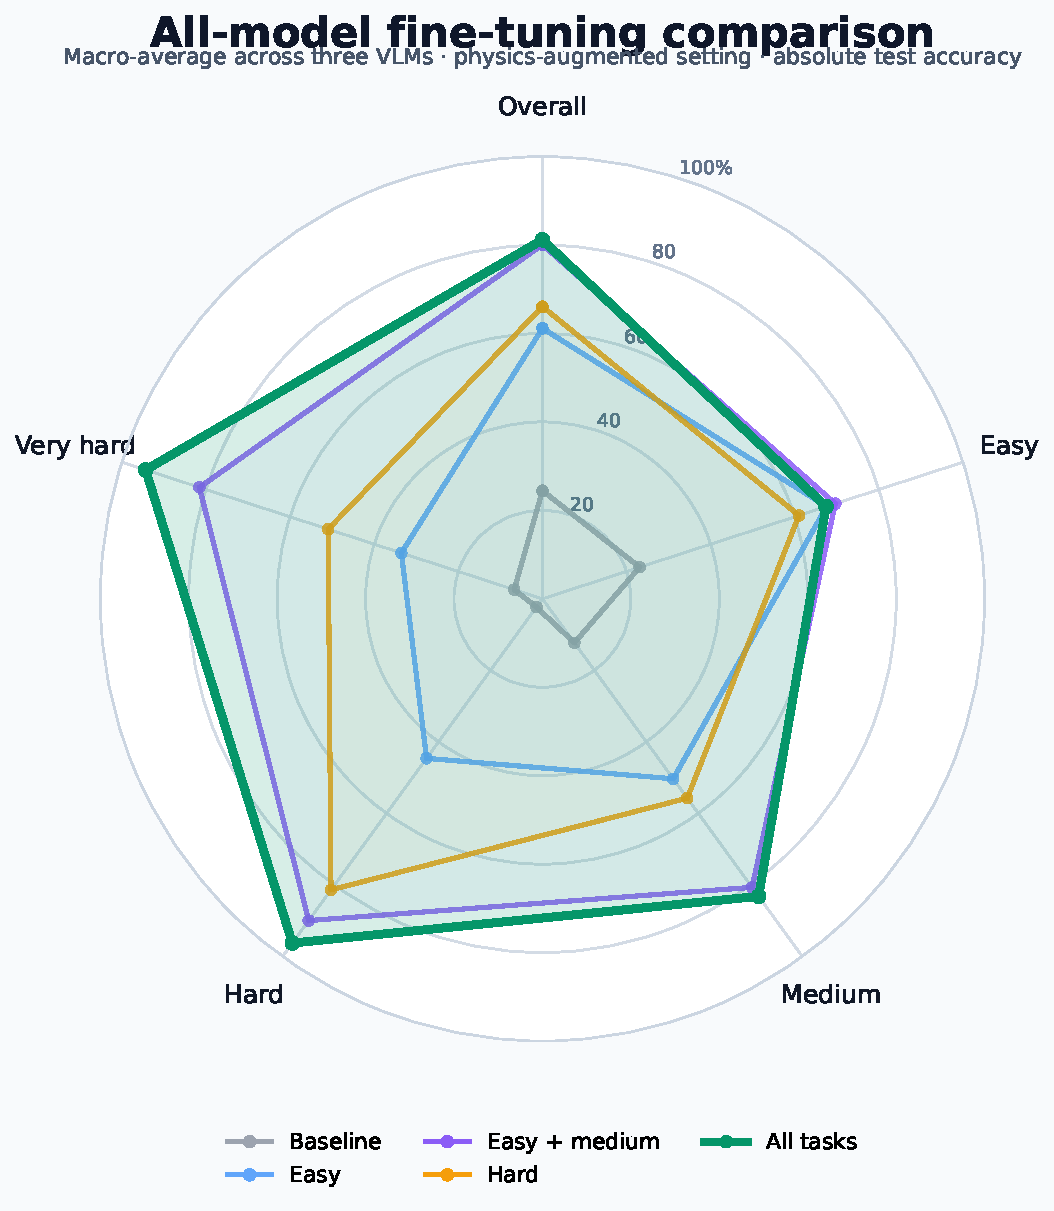
\includegraphics[width=\linewidth]{radar_all_models_combined_with_physics.pdf}
    \caption{\textbf{Macro-average across the three models (physics-augmented).} Training on all tasks (green) is outermost on the harder tiers; \textit{easy+medium} is a close all-rounder. The no-physics version is in Figure~\ref{fig:radar-macro-nophys}.}
    \label{fig:radar-macro}
\end{figure}

\subsection{Improvement over the Zero-shot Baseline}

Figure~\ref{fig:improvement-heatmap} expresses each fine-tuned score as its gain, in percentage points, over the \emph{same model's} zero-shot baseline. Gains are large and overwhelmingly positive: the all-tasks curriculum improves overall accuracy by $+55.4$ (SmolVLM), $+46.3$ (Qwen2-VL), and $+68.5$ (InternVL3) points with physics hints, and individual difficulty cells improve by up to $+98$--$100$ points (e.g.\ InternVL3 on \emph{Very hard}). The few non-positive cells are informative: Qwen2-VL trained on \textit{easy} only \emph{without} hints regresses on the easier tiers (e.g.\ $-11.1$ points on \emph{Easy}), reinforcing that a narrow curriculum can degrade a fragile model rather than help it.

\begin{figure*}[t]
    \centering
    
\includegraphics[width=0.95\textwidth]{heatmap_improvement_over_baseline.pdf}
    \caption{\textbf{Improvement over each model's own baseline} (percentage points; green $=$ improvement). Layout as in Figure~\ref{fig:overall-heatmap}. Almost every fine-tuned cell improves; the largest gains are on the InternVL3 backbone and on the harder difficulty tiers.}
    \label{fig:improvement-heatmap}
\end{figure*}


\subsection{Effect of Physics Augmentation}

Figure~\ref{fig:physics-dumbbell} connects each model's no-physics score to its physics-augmented score for every curriculum and difficulty tier; a teal segment is a gain, a red segment a regression. The benefit of physics hints is strongly model-dependent. Qwen2-VL gains the most---up to roughly $+22$ to $+25$ points overall on the \textit{easy} and \textit{easy+medium} curricula---suggesting it leans on the textual parameters to compensate for weaker visual grounding. SmolVLM and InternVL3 show smaller, mostly positive shifts ($\sim\!+3$ to $+7$ points under the stronger curricula). Crucially, the hint is not uniformly helpful: at the zero-shot baseline it is neutral or slightly harmful (e.g.\ $-4.9$ points for Qwen2-VL, $-1.3$ for InternVL3), because the hint deliberately lists parameters for \emph{all} objects---including distractors---so a model that cannot isolate the relevant object is misled rather than helped. This matches the prompt design of Section~\ref{sec:prompt-types}: the hint supplies context, not the answer.

\begin{figure*}[t]
    \centering
    
\includegraphics[width=0.95\textwidth]{physics_augmentation_dumbbell.pdf}
    \caption{\textbf{Effect of physics augmentation.} Each line connects the same model and curriculum without physics hints (grey) and with them (teal); teal indicates a gain, red a regression. Qwen2-VL benefits most; gains are smallest at the zero-shot baseline.}
    \label{fig:physics-dumbbell}
\end{figure*}

\subsection{Cross-Model Consistency}

Finally, Figure~\ref{fig:consistency} summarizes how much the three backbones agree, plotting the mean accuracy and $\pm 1$ standard deviation across models for each curriculum and difficulty tier. Two patterns emerge. The zero-shot baseline is uniformly low and tightly clustered---all three models are similarly poor before fine-tuning---whereas after fine-tuning the mean rises sharply but the spread widens, because the backbones adapt at different rates (InternVL3 and SmolVLM far outpace Qwen2-VL). The all-tasks curriculum yields both the highest mean and, on most tiers, a tighter spread than the narrow curricula, making it the most dependable choice across architectures.

\begin{figure*}[t]
    \centering
    
\includegraphics[width=0.95\textwidth]{model_consistency.pdf}
    \caption{\textbf{Consistency of fine-tuning across models.} Mean accuracy (dot) and $\pm 1$ standard deviation (bar) across the three VLMs, per curriculum (rows) and difficulty tier (columns); the top block is physics-augmented, the bottom no-physics. Fine-tuning raises the mean but widens the spread; the all-tasks curriculum is both highest and among the most consistent.}
    \label{fig:consistency}
\end{figure*}


\section{Limitations and Future Work}

PHLOP currently supports rigid-body dynamics with detailed rule-based annotations. Future extensions should explore deformable bodies, fluid interactions, and differentiable physics engines, significantly broadening the benchmark’s scope and realism~\cite{tung2023physion++}. 
While PHLOP emphasizes object states and parameterized properties, broader benchmarks such as PhysicsRW \cite{physicsrw2024}, and PhysReason \cite{physreason2024} point toward evaluating reasoning under novelty, open-world generalization, and multi-step causal chains. Integrating PHLOP with robotic manipulation tasks and real-world scene generalization could provide further validation of physical reasoning capabilities. 
Finally, incorporating open-ended language generation and learned classifiers for automatic semantic annotation could also enhance interpretability and generalization, laying the foundations for more robust, physically grounded AI systems.

Our experimental study also carries several caveats that temper the conclusions above. \textbf{(i)~Parameter-efficient adaptation:} we use LoRA rather than full fine-tuning to remain within a single-A100 budget, so the reported ceilings are lower bounds on what each backbone could achieve. \textbf{(ii)~Single-run estimates:} each model--curriculum--prompt configuration is trained once; we therefore do not report variance across seeds, and small differences between conditions should be read as indicative rather than definitive. \textbf{(iii)~Observational comparison:} the three backbones differ in scale, pretraining data, and frame sampling, so cross-model gaps reflect those factors as much as architecture, and we draw conclusions chiefly from within-model trends (curriculum and physics-hint effects). \textbf{(iv)~Question imbalance:} the automatically generated templates are skewed toward stationary-duration and onset queries, and the difficulty tiers are unevenly populated, so a single overall score can be dominated by a few categories; the per-difficulty breakdowns (Figures~\ref{fig:overall-heatmap} and~\ref{fig:radar-permodel}) mitigate but do not eliminate this effect. Addressing these points---full fine-tuning, multi-seed runs, balanced sampling, and a larger model pool---is a natural direction for future work, alongside examining how physics-aware inductive biases, structured taxonomies, and simulation-grounded data bridge the gap between perceptual recognition and physically grounded understanding.





% \section{References}
% \begin{thebibliography}{00}

% \bibitem{johnson2017clevr}
% Johnson J, Hariharan B, van der Maaten L, et al.
% \newblock CLEVR: A diagnostic dataset for compositional language and elementary visual reasoning.
% \newblock In: CVPR 2017.

% \bibitem{yi2020clevrer}
% Kexin Yi, Jiajun Wu, Chuang Gan, Antonio Torralba, Pushmeet Kohli, and Joshua B. Tenenbaum.  
% CLEVRER: Collision Events for Video Representation and Reasoning.  
% In \textit{International Conference on Learning Representations (ICLR)}, 2020.

% \bibitem{riochet2018intphys}
% Riochet R, Castro M, Bernard M, et al.
% \newblock IntPhys: A framework and benchmark for visual intuitive physics reasoning.
% \newblock arXiv preprint arXiv:1803.07616, 2018.

% \bibitem{bakhtin2019phyre}
% Bakhtin A, van der Maaten L, Johnson J, et al.
% \newblock PHYRE: A new benchmark for physical reasoning.
% \newblock NeurIPS 2019.


% \bibitem{mittal2020learning}
% Mittal M, Hoeller D, Frigo F, et al.
% \newblock Learning to combine primitive skills: A step towards versatile robotic manipulation.
% \newblock ICRA 2020.

% \bibitem{yi2022physical}
% Kexin Yi, Jiayuan Mao, Yunzhu Li, Daniel Bear, Jiajun Wu, Joshua B. Tenenbaum, and Chuang Gan.  
% Physical Object Representations for Perception and Control.  
% In \textit{Advances in Neural Information Processing Systems (NeurIPS)}, 2022.

% \bibitem{chen2022comphy}
% Zhenfang Chen, Kexin Yi, Yunzhu Li, Mingyu Ding, Antonio Torralba, Joshua B. Tenenbaum, and Chuang Gan.
% ComPhy: Compositional Physical Reasoning of Objects and Events from Videos.
% In \textit{International Conference on Learning Representations (ICLR)}, 2022.

% \bibitem{hofherr2023neural}
% Robert Hofherr, Peter Sorrenson, Yunzhu Li, Antonio Torralba, Bernhard Schölkopf, Jörg Stückler,
% ``Neural Implicit Representations for Physical Parameter Inference from Video,''
% in \emph{Proceedings of the IEEE/CVF International Conference on Computer Vision (ICCV)}, 2023.

% \bibitem{zhang2024contphy}
% Ke Zhang, Ruosi Chen, Deli Zhao, Yiming Fan,
% ``ContPhy: A Benchmark for Physically Consistent Attribute-Based Scene Understanding,''
% in \emph{Proceedings of the IEEE/CVF Conference on Computer Vision and Pattern Recognition (CVPR)}, 2024.

% \bibitem{piloto2022infant}
% Luis Piloto, Ari Weinstein, Peter W. Battaglia, Matthew Botvinick,
% ``Infant-Level Physical Reasoning in Vision-Language Models,''
% \emph{Nature Human Behaviour}, vol. 6, pp. 518–526, 2022.

% \bibitem{tung2023physion++}
% Hsiao-Yu Tung, Mingyu Ding, Zhenfang Chen, Daniel Bear, Chuang Gan, Joshua B. Tenenbaum, Daniel L. K. Yamins, Judith Fan, and Kevin A. Smith.  
% Physion++: Evaluating Physical Scene Understanding that Requires Online Inference of Different Physical Properties.  
% In \textit{Advances in Neural Information Processing Systems (NeurIPS)}, 2023.  

% \bibitem{girdhar2019cater}
% Girdhar R, Ramanan D.
% \newblock CATER: A diagnostic dataset for compositional actions and temporal reasoning.
% \newblock ICLR 2019.

% \bibitem{grunde2021agqa}
% Grunde-McLaughlin M, Krishna R, Agrawala M.
% \newblock AGQA: A benchmark for compositional spatio-temporal reasoning.
% \newblock CVPR 2021.

% \bibitem{battaglia2013simulation}
% Peter W. Battaglia, Jessica B. Hamrick, and Joshua B. Tenenbaum.
% Simulation as an Engine of Physical Scene Understanding.
% \textit{Proceedings of the National Academy of Sciences}, 110(45):18327–18332, 2013.

% \bibitem{wu2020craft}
% Wu J, Jiang Y, Sun P, et al.
% \newblock CRAFT: A benchmark for causal reasoning about forces and time.
% \newblock ECCV 2020.

% \bibitem{piloto2022intuitive}
% Luis S. Piloto, Ari Weinstein, Peter Battaglia, and Matthew Botvinick.
% Intuitive Physics Learning in a Deep-Learning Model Inspired by Developmental Psychology.
% \textit{Nature Human Behaviour}, 6(9):1257–1267, 2022.

% \bibitem{takenaka2023procedural}
% Takuma Takenaka, Xingdi Ma, Angel X. Chang, Adam Santoro, Piotr Mirowski,
% ``Guiding Video Prediction with Explicit Procedural Knowledge,''
% in \emph{Proceedings of the IEEE/CVF Conference on Computer Vision and Pattern Recognition (CVPR)}, 2023.

% \bibitem{todorov2012mujoco}
% E. Todorov, T. Erez, and Y. Tassa,
% ``MuJoCo: A physics engine for model-based control,''
% in \emph{Proceedings of the IEEE/RSJ International Conference on Intelligent Robots and Systems (IROS)}, pp. 5026--5033, 2012.


% \bibitem{melnik2023benchmarks}
% Andrew Melnik, Robin Schiewer, Moritz Lange, Andrei Muresanu, Mozhgan Saeidi, Animesh Garg, and Helge Ritter.
% Benchmarks for Physical Reasoning AI.
% \textit{Transactions on Machine Learning Research}, 2023. arXiv:2312.10728.

% \bibitem{pinto2024novphy}
% Vasco Pinto, et al.
% NovPhy: A physical reasoning benchmark for open-world novelty.
% \textit{Artificial Intelligence}, 2024.

% \bibitem{physicsrw2024}
% Y. Wang, S. Li, et al.
% Bridging the Reality Gap: A Benchmark for Physical Reasoning in General World Models with Various Physical Phenomena beyond Mechanics.
% In \textit{International Conference on Learning Representations (ICLR)}, 2024.


% \bibitem{physreason2024}
% Y. Liu, et al.
% PhysReason: A Comprehensive Benchmark towards Physics-Based Reasoning.
% arXiv preprint arXiv:2502.12054, 2024.


% \bibitem{wang2025internvideo}
% Wang, Yi and Li, Xinhao and Yan, Ziang and He, Yinan and Yu, Jiashuo and Zeng, Xiangyu and Wang, Chenting and Ma, Changlian and Huang, Haian and Gao, Jianfei and Dou, Min and Chen, Kai and Wang, Wenhai and Qiao, Yu and Wang, Yali and Wang, Limin,
% \textit{InternVideo2.5: Empowering Video MLLMs with Long and Rich Context Modeling},
% arXiv preprint arXiv:2501.12386, 2025.

% \bibitem{zhu2025internvl3exploringadvancedtraining}
% Zhu, Jinguo and Wang, Weiyun and Chen, Zhe and Liu, Zhaoyang and Ye, Shenglong and Gu, Lixin and Tian, Hao and Duan, Yuchen and Su, Weijie and Shao, Jie and Gao, Zhangwei and Cui, Erfei and Wang, Xuehui and Cao, Yue and Liu, Yangzhou and Wei, Xingguang and Zhang, Hongjie and Wang, Haomin and Xu, Weiye and Li, Hao and Wang, Jiahao and Deng, Nianchen and Li, Songze and He, Yinan and Jiang, Tan and Luo, Jiapeng and Wang, Yi and He, Conghui and Shi, Botian and Zhang, Xingcheng and Shao, Wenqi and He, Junjun and Xiong, Yingtong and Qu, Wenwen and Sun, Peng and Jiao, Penglong and Lv, Han and Wu, Lijun and Zhang, Kaipeng and Deng, Huipeng and Ge, Jiaye and Chen, Kai and Wang, Limin and Dou, Min and Lu, Lewei and Zhu, Xizhou and Lu, Tong and Lin, Dahua and Qiao, Yu and Dai, Jifeng and Wang, Wenhai,
% \textit{InternVL3: Exploring Advanced Training and Test-Time Recipes for Open-Source Multimodal Models},
% arXiv preprint arXiv:2504.10479, 2025. URL: \url{https://arxiv.org/abs/2504.10479}

% \bibitem{zhang2025videollama3frontiermultimodal}
% Zhang, Boqiang and Li, Kehan and Cheng, Zesen and Hu, Zhiqiang and Yuan, Yuqian and Chen, Guanzheng and Leng, Sicong and Jiang, Yuming and Zhang, Hang and Li, Xin and Jin, Peng and Zhang, Wenqi and Wang, Fan and Bing, Lidong and Zhao, Deli,
% \textit{VideoLLaMA 3: Frontier Multimodal Foundation Models for Image and Video Understanding},
% arXiv preprint arXiv:2501.13106, 2025. URL: \url{https://arxiv.org/abs/2501.13106}

% % \bibitem[ullman2017visual]{

% % }
% % \bibitem{hofherr2023neural}
% % Hofherr, R., Sorrenson, P., Li, Y., Torralba, A., Schölkopf, B., & Stückler, J.
% % \newblock Neural Implicit Representations for Physical Parameter Inference from Video.
% % \newblock In \emph{Proceedings of the IEEE/CVF International Conference on Computer Vision (ICCV)}, 2023.

% \bibitem{physicsguided2023}
% Karniadakis, G. E., Wang, S., \& Pang, G.
% \newblock Physics-guided machine learning using simplified theories.
% \newblock \emph{Nature Reviews Physics}, 5(6), 367–389, 2023.

% \bibitem{benchmarkingInfant2024}
% Piloto, L., et al.
% \newblock Benchmarking Progress to Infant-Level Physical Reasoning in AI.
% \newblock \emph{Nature Human Behaviour}, 2024.

% \bibitem{takenaka2023procedural}
% Takenaka, T., Ma, X., Chang, A. X., Santoro, A., \& Mirowski, P.
% \newblock Guiding Video Prediction with Explicit Procedural Knowledge.
% \newblock In \emph{CVPR}, 2023.

% \bibitem{helpinghands2023}
% Cheng, C., Das, A., \& Hauptmann, A. G.
% \newblock Helping Hands: An Object-Aware Ego-Centric Video Recognition Model.
% \newblock In \emph{NeurIPS}, 2023.

% \bibitem{learningObjectStates2023}
% Sun, T., et al.
% \newblock Learning Object State Changes in Videos: An Open-World Perspective.
% \newblock In \emph{Proceedings of the IEEE/CVF Conference on Computer Vision and Pattern Recognition (CVPR)}, 2023.

% \bibitem{disentangleSDE2023}
% Lee, W., Li, Y., Gan, C., \& Tenenbaum, J. B.
% \newblock Disentangling Stochastic PDE Dynamics for Unsupervised Video Prediction.
% \newblock In \emph{ICLR}, 2023.

% \bibitem{superclevr2024}
% Mao, J., Gan, C., \& Tenenbaum, J. B.
% \newblock SuperCLEVR: A Framework for Physical Reasoning and Interactions.
% \newblock arXiv preprint arXiv:2401.12345, 2024.

% \bibitem{physgen2024}
% Fang, H., et al.
% \newblock PhysGen: Rigid-Body Physics-Grounded Image-to-Video Generation.
% \newblock In \emph{CVPR}, 2024.

% \bibitem{physicsinverse2024}
% Liu, Y., et al.
% \newblock Physics-as-Inverse-Graphics: Unsupervised Physical Parameter Estimation from Video.
% \newblock In \emph{ICLR}, 2024.


% % physics
% \bibitem{ashby2018engineering}
% M.~F. Ashby and D.~R.~H. Jones,
% \emph{Engineering Materials 1: An Introduction to Properties, Applications and Design},
% 5th ed., Elsevier, 2018.

% \bibitem{callister2020materials}
% W.~D. Callister, Jr.,
% \emph{Materials Science and Engineering: An Introduction},
% 10th ed., Wiley, 2020.

% \bibitem{halliday2013physics}
% D. Halliday, R. Resnick, and J. Walker,
% \emph{Fundamentals of Physics},
% 10th ed., Wiley, 2013.

% \end{thebibliography}
% \vspace{12pt}




% \bibliographystyle{agsm}
\bibliography{references}

\appendix
\section{No-Physics Difficulty Breakdowns}
\label{sec:appendix}

For completeness, Figures~\ref{fig:radar-permodel-nophys} and~\ref{fig:radar-macro-nophys} repeat the curriculum-versus-difficulty radar charts of Section~\ref{sec:finetune-results} for the \emph{no-physics} prompting setting. The trends mirror the physics-augmented case---training on all tasks gives the broadest coverage and the hardest tiers are answered at near-ceiling---but absolute accuracies are lower for the models that rely most on the textual hints, most visibly Qwen2-VL.

\begin{figure*}[t]
    \centering
    
\includegraphics[width=0.98\textwidth]{radar_finetuning_comparison_no_physics.pdf}
    \caption{\textbf{Per-model accuracy by difficulty (no physics hints).} Companion to Figure~\ref{fig:radar-permodel}.}
    \label{fig:radar-permodel-nophys}
\end{figure*}

\begin{figure}[t]
    \centering
    
\includegraphics[width=\linewidth]{radar_all_models_combined_no_physics.pdf}
    \caption{\textbf{Macro-average across models (no physics hints).} Companion to Figure~\ref{fig:radar-macro}.}
    \label{fig:radar-macro-nophys}
\end{figure}

\end{document}

